\chapter{Ignitions}
\label{ch:ignitions}


 \begin{marginfigure}[3cm]
	\begin{center}
		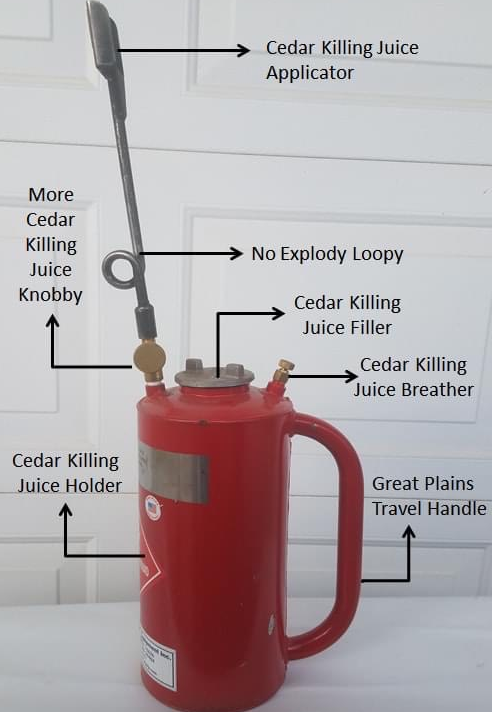
\includegraphics[width=2.2in]
		{ops/ignitions/DripTorchDiagram}
		\ImageCredit{Nebraska Prescribed Fire Council, via Facebook}
		\caption{Important components of the drip torch, with special reference to maintaining open grassland in the US Great Plains.
\label{fig:DripTorchDiagram} } 
		% (Fig.~\ref{fig:DripTorchDiagram})
	\end{center}
\end{marginfigure}

Most prescribed burns are deliberately started by humans with incendiary devices.%\footnote{Under the broader concept of \emph{wildland fire use} a prescription might also apply to a natural ignition in a wilderness area, allowing it to ``let burn'' under a specific set of conditions and/or within a specific area.} 
Tactically, these devices provide for the controlled firing of wildland fuels. 
Strategically, their operation can serve broad objectives such as fire behavior, fire effects, and smoke management. 
As such, wildland fire ignitions combine science and art. 

The most common firing device is the \emph{drip torch} (Fig.~\ref{fig:DripTorchDiagram}). 
While several configurations are available, each are essentially a handheld tank of liquid fuel with a wick that allows a small amount of fuel to pass over the burning wick, ignite, and carry fire to the fuelbed (Figs.~\ref{fig:IgnitionDevices}~\&~\ref{fig:FillingTorches}). 
Several other devices are basically extensions of the same principle\textemdash moving liquid fuel over a burning wick\textemdash and include vehicle-mounted torches with large-capacity tanks and fuel pumps for extended range (Fig.~\ref{fig:IgnitionDevices}, \emph{center}). 

Another major class of firing devices includes those that launch, propel, or release flares or fuel capsules containing a special mix of chemicals (e.g., potassium permanganate \& glycol) that, once combined, slowly undergo a reaction that eventually releases enough heat to ignite vegetation (Fig.~\ref{fig:IgnitionDevices}, \emph{right}). 
Capsules are launched via handheld devices or dropped from helicopters and drones.
Such devices enable remote ignitions, when physically standing in or near the fuel is difficult or hazardous. 



\begin{figure} 
	\begin{center}
		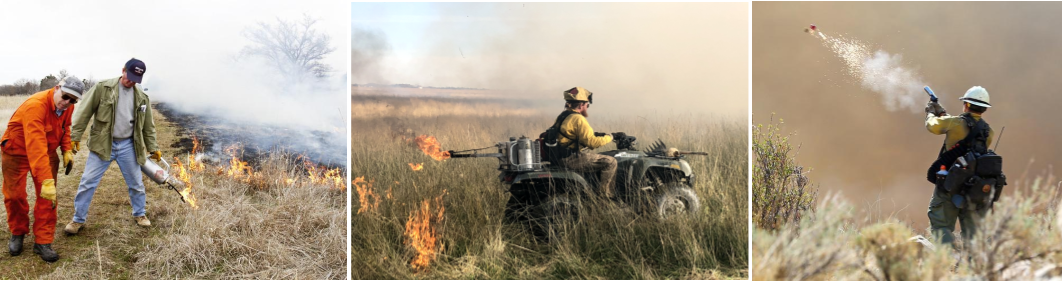
\includegraphics[width=1\textwidth]
		{ops/ignitions/IgnitionDevices}
		\ImageCredit{L: Noble Research Foundation, CC BY-NC-ND 2.0; C: Carissa Wonkka; R: Geoff Liesik, BLM, public domain}
		\ImageIndex{CC BY-NC-ND 2.0}
		{fig:SlingPsychrometer}
		{Noble Research Foundation}
		{https://www.flickr.com/photos/noblefoundation/6775182446}
	\end{center}
	\caption{L: The drip torch is the primary source of prescribed fire ignitions. C: ATV-mounted torches facilitate faster firing. 
	R: A pistol-style flare launcher fired by a member of the Wolf Creek Hotshots on the Bear Fire near Helper, Utah. 
	Such devices facilitate remote ignitions. 
	} \label{fig:IgnitionDevices}
	%(Fig.~\ref{fig:IgnitionDevices})
\end{figure}

\section{Ignition patterns} 

 \begin{marginfigure}
	\begin{center}
		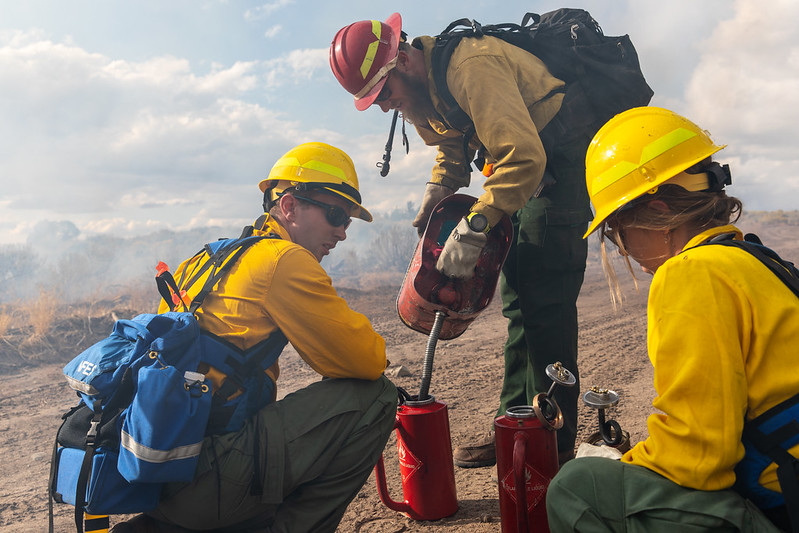
\includegraphics[width=2.2in]
		{ops/ignitions/FillingTorches}
		% \ImageCredit{ }
		\caption{Drip torches are filled with liquid fuel, sometimes kerosene, but often a mix of 40\% gasoline and 60\% diesel fuel. 
			The gasoline provides rapid ignition at the wick, while oil in the diesel allows the fuel to burn long enough to transfer heat to vegetation.
			\label{fig:FillingTorches} } 
		% (Fig.~\ref{fig:FillingTorches})
	\end{center}
\end{marginfigure}

Perhaps the most determinant factor for prescribed fire effectiveness and operational safety is the way ignitions are applied to the burn unit, known as the \emph{ignition pattern}. 
Because wind is so important to fire intensity and spread, almost all ignition plans are made with reference to wind direction (Fig.~\ref{fig:IgnitionPatterns}). 
Topographic effects and potential impacts within and beyond the burn unit also influence the ignition pattern, such as which side of a unit is best to start firing from, and which direction(s) smoke must not be allowed to travel. 
Combining these two elements defines the acceptable wind directions for a given unit\textemdash some burn units might be so simple and hazard-free that they can be burned on days with wind coming from any direction, whereas some units have such a high degree of complexity that managers would only begin firing if the wind was from a specific direction.   

\begin{figure} 
	\begin{center}
		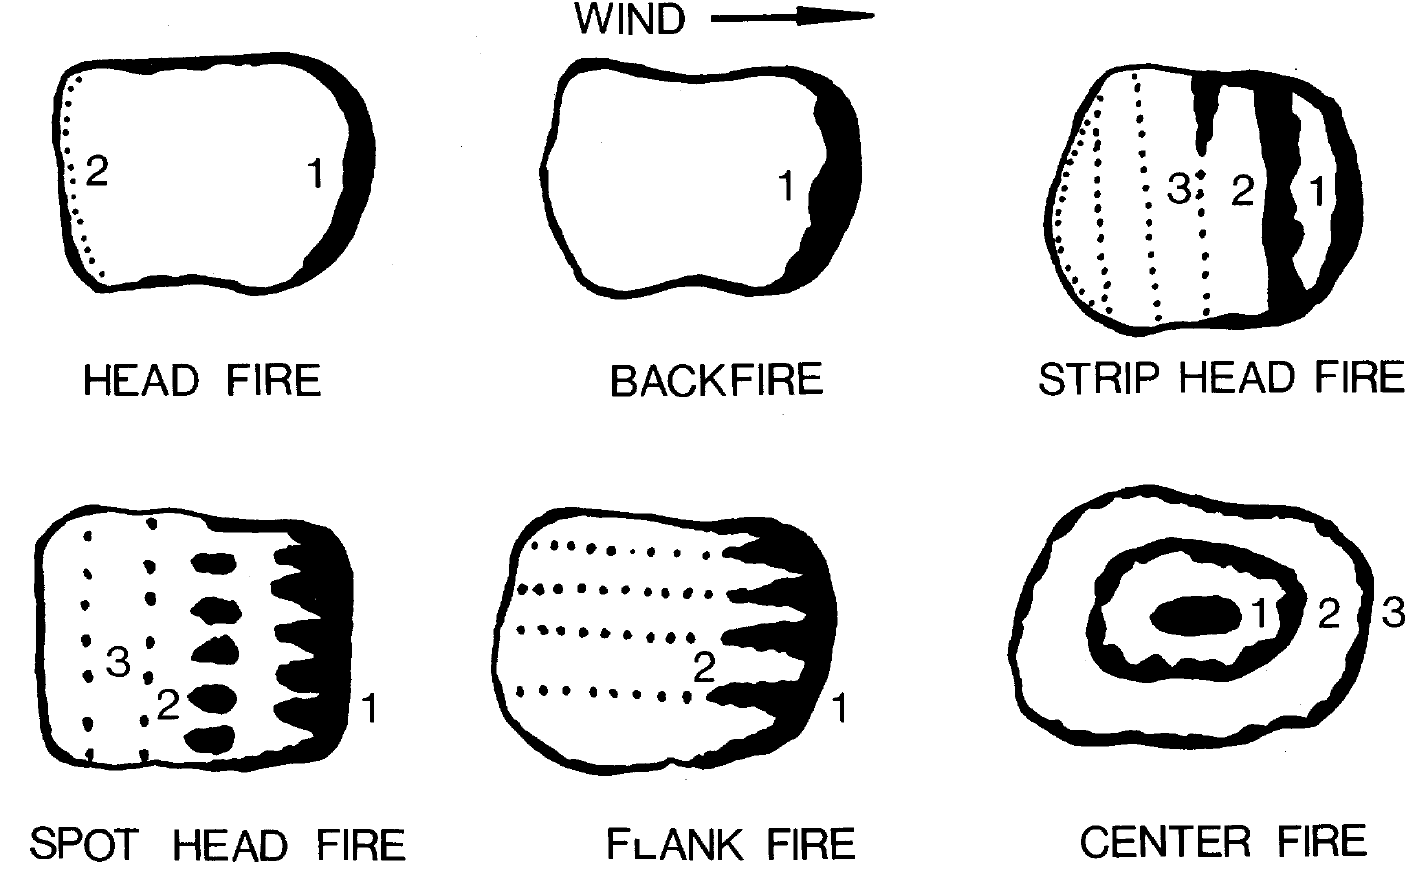
\includegraphics[width=1\textwidth]
		{ops/ignitions/IgnitionsMartinDell}
	\end{center}
	\caption{Six ignition patterns for prescribed fire \citep{martin1978}. 
		Numerals indicate order of firing. 
		The center fire pattern is often applied as a spiral, with a single ignition operator beginning in the center of the unit and circling out to the edges. 
		This facilitates, on the scale of the entire burn unit, the sort of convective ``pull'' illustrated below. 
	 \label{fig:IgnitionPatterns} }
	%(Fig.~\ref{fig:IgnitionPatterns})
\end{figure}

Within the unit, the pattern of ignition is generally chosen based on desired fire effects and limitations on spread. 
Broadly speaking, patterns facilitate (a) faster, more intense head fires that move with the wind; (b) slower-moving backing fires that might have longer residence time as they creep against the wind; or (c) a series of flanking fires that spread perpendicularly to the wind and combine behavior and heating properties of both head and backing fires (Fig.~\ref{fig:IgnitionPatterns}). 
The number and spacing of strips and spots can be varied to regulate the direction and amount of smoke emissions and the time it takes to completely burn the unit.

\begin{marginfigure} 
	\begin{center}
		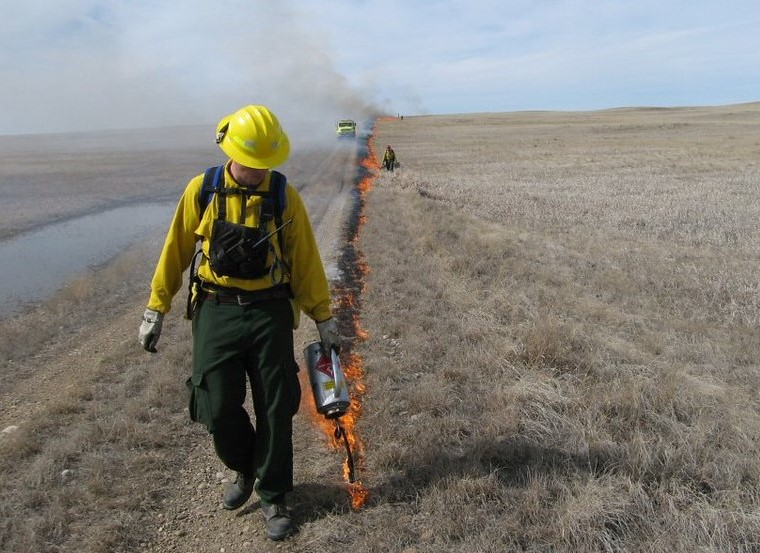
\includegraphics[width=2.2in]
		{ops/ignitions/PrimaryTorchLine}
	\end{center}
	\caption{A primary torch operator starts a back burn from right along the fire break, which in this case is a two-track road with gravel and low vegetation accessible by pumper vehicles for holding the fire within the unit. 
	 \label{fig:PrimaryTorch} }
	%(Fig.~\ref{fig:PrimaryTorch})
\end{marginfigure}

Almost every ignition pattern begins with a line of fire placed perpendicular to the wind on the downwind side of the unit (Fig.~\ref{fig:IgnitionPatterns}). 
Because the wind is pushing this fire away from the area intended to be burned line is typically ran along a robust fire break that combines (a) low or no fuels beyond the edge of the burn unit with (b) accessibility to vehicles that can suppress fire and patrol the line (Fig.~\ref{fig:PrimaryTorch}). 

\begin{figure}[t] 
	\begin{center}
		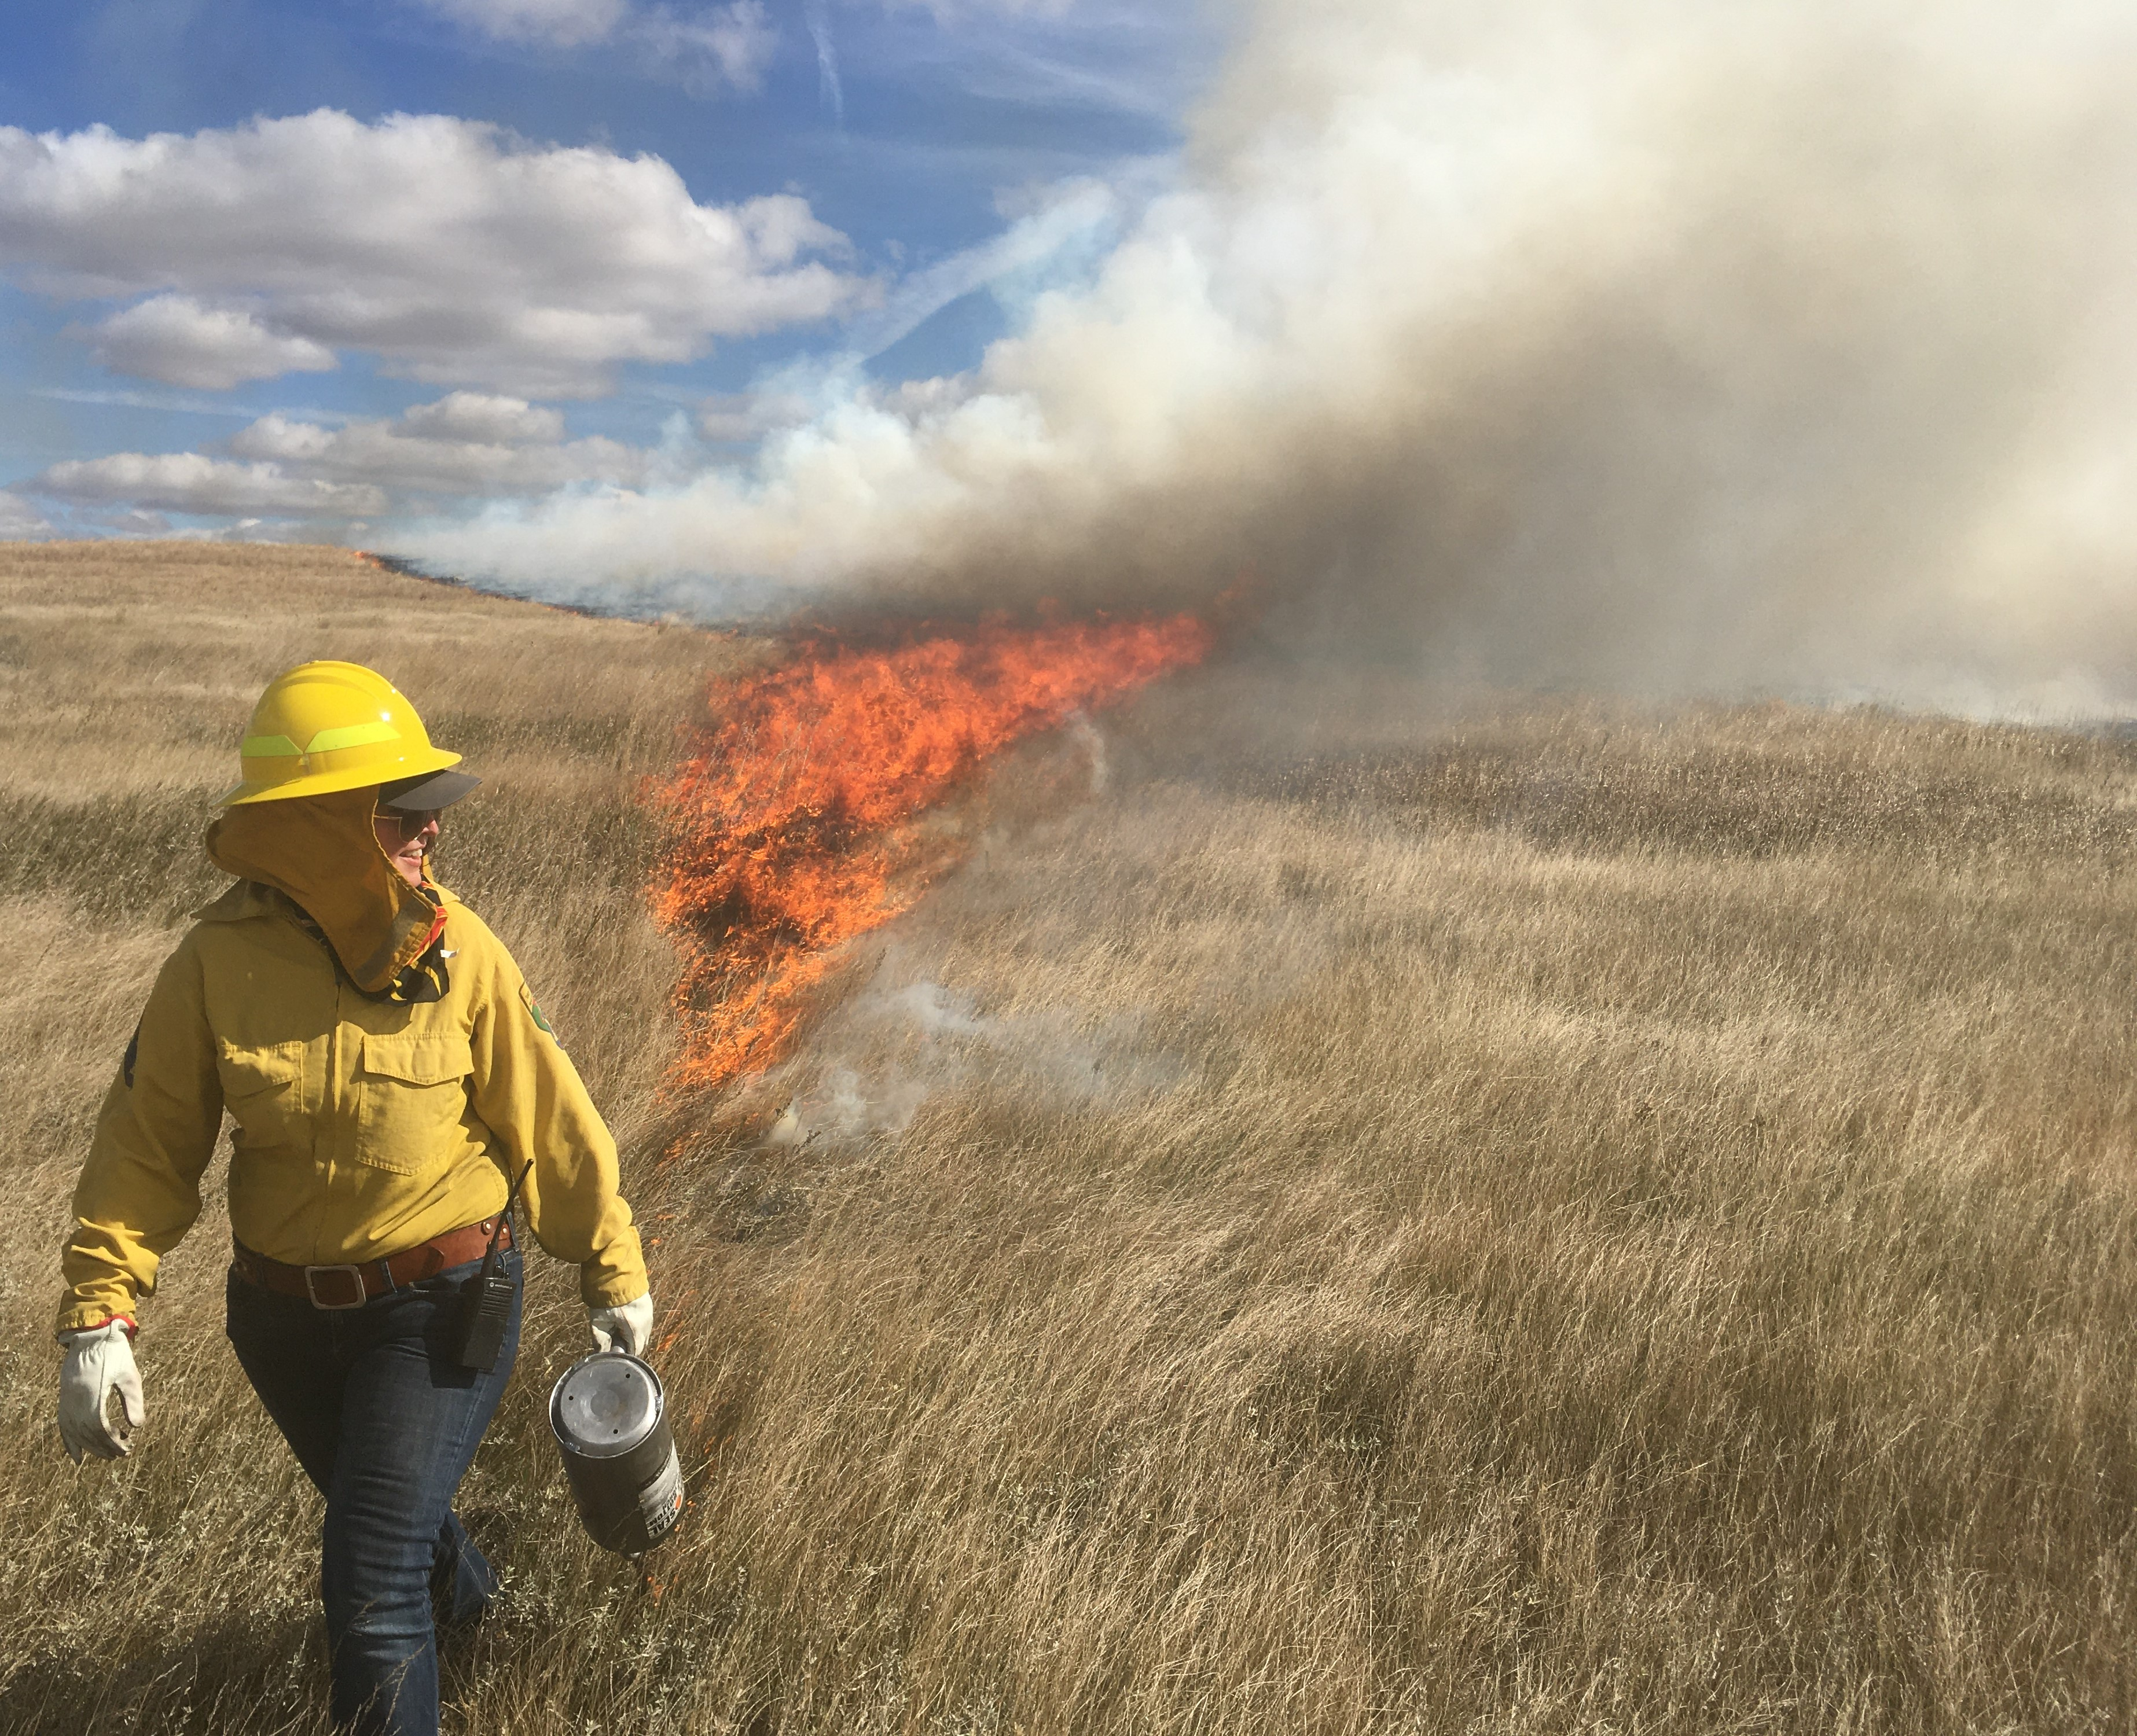
\includegraphics[width=0.465\textwidth]
		{ops/ignitions/WonkkaStrips}~
		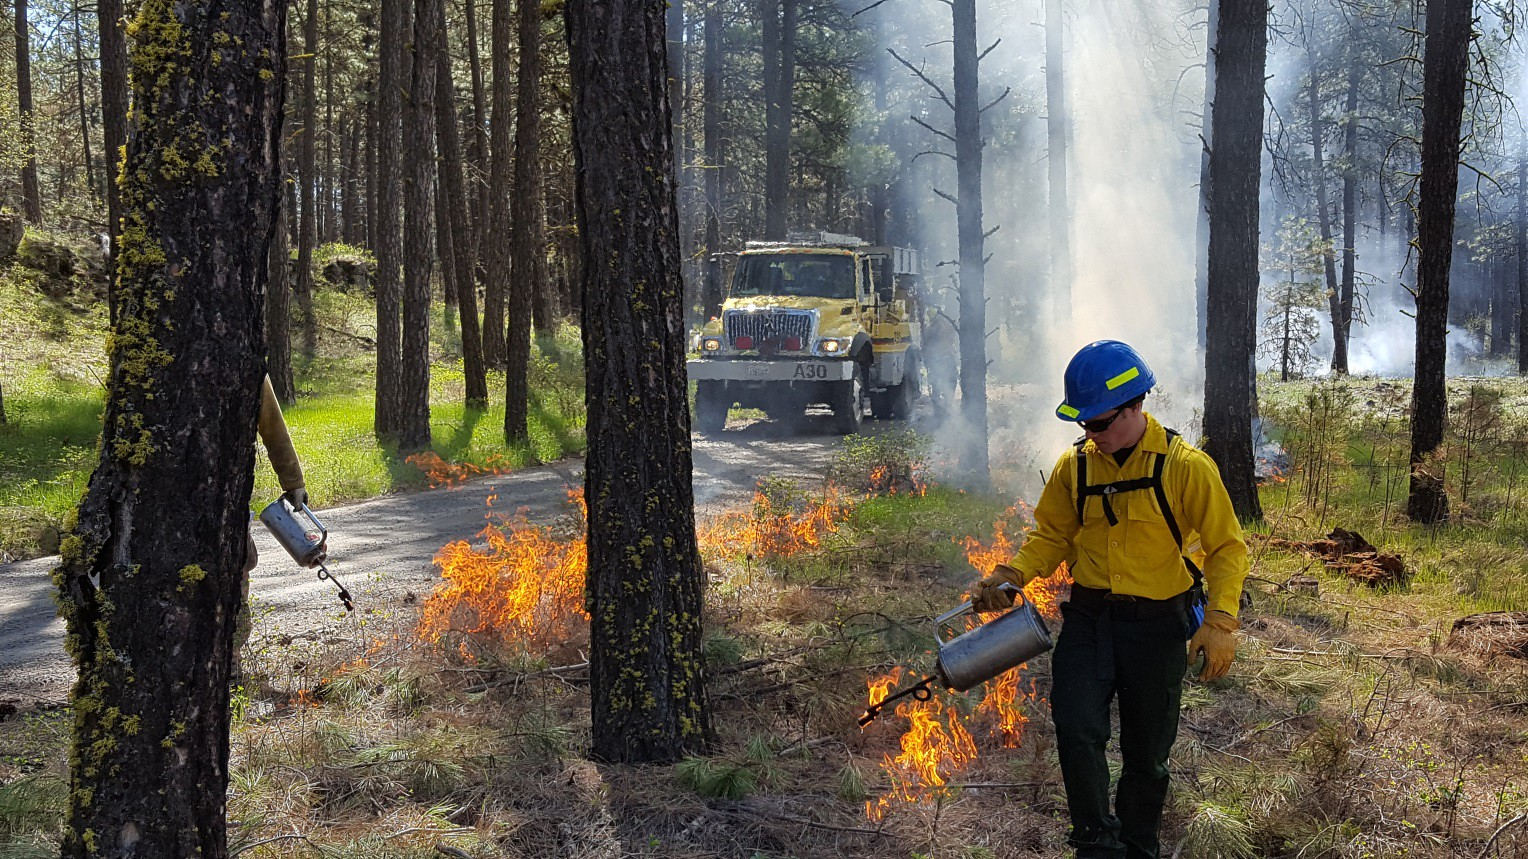
\includegraphics[width=0.535\textwidth]
		{ops/ignitions/SecondaryTorchWoods}
	\end{center}
	\caption{\emph{Left:} Dr. Carissa Wonkka lays a strip head fire through a grassland fuelbed to both widen the ``black'' downwind but also lift the smoke column off the control lines to make live better for holding crew. 
		\emph{Right:} A secondary torch operator lays a strip inside of the primary operator, who is firing off the road. 
		An engine supports holding behind the torches as they move forward. 
		\label{fig:SecondaryTorch} }
	%(Fig.~\ref{fig:SecondaryTorch})
\end{figure}

\begin{marginfigure} 
	\begin{center}
		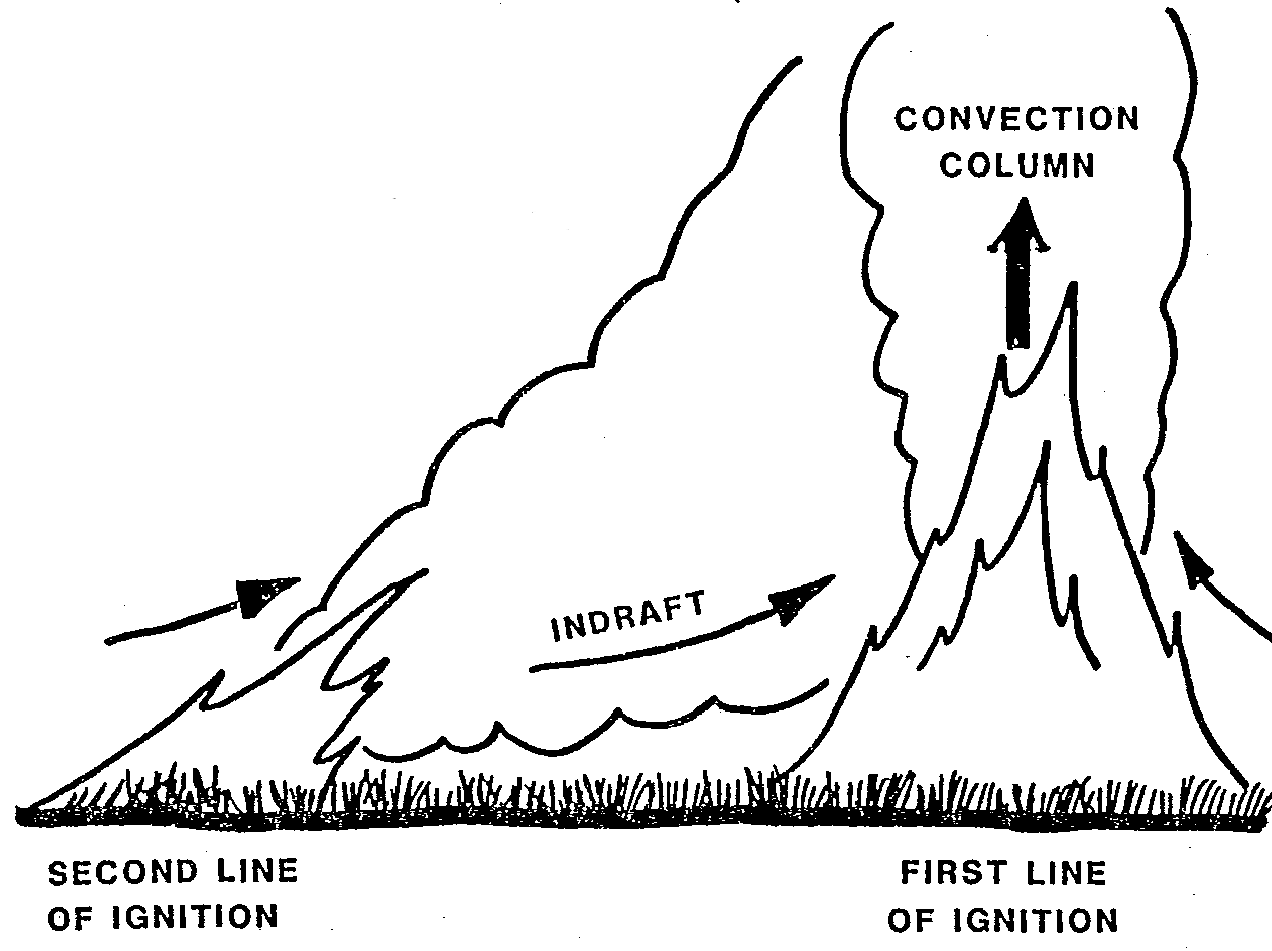
\includegraphics[width=2.2in]
		{ops/ignitions/RothermelSecondary}
			\ImageCredit{\citet{rothermel1984}}
	\end{center}
	\caption{Under good convective conditions, two parallel strip fires will interact.
		The primary line, burning more intensely as it has been burning longer, will ``pull'' the secondary line in towards it, which enhances control by limiting the outward rate of spread. 
		Meanwhile, the secondary line will draw the convective column into the unit, allowing smoke to ventilate more vertically and keep it above crewmembers working on the line.   
		\label{fig:rothermel1984} }
	%(Fig.~\ref{fig:rothermel1984})
\end{marginfigure}

As the burn crew works to develop control lines around the entire burn unit\textemdash widening fire breaks with burned-out areas to increase the distance between flames and embers from the unit and fuels beyond the edges of the unit\textemdash additional torch operators are often deployed within the burn unit (Fig.~\ref{fig:SecondaryTorch}). 
These secondary torch operators lay \emph{strip ignitions} that not only increase the burned area by widening the lines faster, but under good convective conditions actually influence the interaction between the prescribed fire and the atmosphere (Fig.~\ref{fig:rothermel1984}). 

Under very good convective conditions, the smoke columns of distant flame fronts will interact in the atmosphere (Fig.~\ref{fig:PlumesConverge}). 
These interactions can temporarily change the direction and rate of spread, reducing the relative influence of wind. 
At very broad scales, such as large wildfires, the driver of spread rate and direction can shift from wind to convention, creating a \emph{plume-driven fire}. 

\begin{figure}[b]
	\begin{center}
		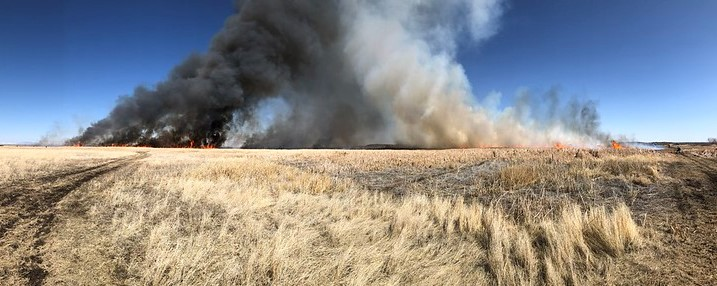
\includegraphics[width=1\textwidth]
		{ops/ignitions/PlumesConverge}
		\ImageCredit{Austin Catlin, BLM, public domain}
	\end{center}
	\caption{A remarkable image of two plumes converging on the Market Lake Prescribed Fire in eastern Idaho.
	The lighter smoke is from light fuels (e.g., grass) that fully combusted. 
	The darker smoke is due to heavier fuels pulled aloft prior to complete combustion and/or combustion of secondary compounds in the vegetation (e.g., sagebrush). 
	} \label{fig:PlumesConverge}
	%(Fig.~\ref{fig:PlumesConverge})
\end{figure}